\documentclass[11pt]{article}
\usepackage{coling2014}
\usepackage{times}
\usepackage{url}
\usepackage{latexsym}
\usepackage{graphicx}


\usepackage{fontspec}
\usepackage{xunicode}
\usepackage{xltxtra}

\usepackage{graphicx}
\usepackage{caption}
\usepackage{subcaption}

\title{Hyper-minimization of Finite state Lexicions Using Flag Diacritics}


\author{First Author \\
  Affiliation / Address line 1 \\
  Affiliation / Address line 2 \\
  Affiliation / Address line 3 \\
  {\tt email@domain} \\\And
  Second Author \\
  Affiliation / Address line 1 \\
  Affiliation / Address line 2 \\
  Affiliation / Address line 3 \\
  {\tt email@domain} \\}

\date{}

\begin{document}
\maketitle
\begin{abstract}
  max 200 words
\end{abstract}




\section{Introduction}
%
% The following footnote without marker is needed for the camera-ready
% version of the paper.
% Comment out the instructions (first text) and uncomment the 8 lines
% under "final paper" for your variant of English.
% 
\blfootnote{
    %
    % for review submission
    %
    %\hspace{-0.65cm}  % space normally used by the marker
    %Place licence statement here for the camera-ready version, see
    %Section~\ref{licence} of the instructions for preparing a
    %manuscript.
    %
    % % final paper: en-uk version (to license, a licence)
    %
    % \hspace{-0.65cm}  % space normally used by the marker
    % This work is licensed under a Creative Commons 
    % Attribution 4.0 International Licence.
    % Page numbers and proceedings footer are added by
    % the organisers.
    % Licence details:
    % \url{http://creativecommons.org/licenses/by/4.0/}
    % 
    % % final paper: en-us version (to licence, a license)
    %
     \hspace{-0.65cm}  % space normally used by the marker
     This work is licenced under a Creative Commons 
     Attribution 4.0 International License.
     Page numbers and proceedings footer are added by
     the organizers.
     License details:
     \url{http://creativecommons.org/licenses/by/4.0/}
}

Finite-state transducers are an established way of encoding
morphological analysers for natural languages. Nevertheless,
full-scale morphological analysers can often grow to be too large for
use cases like spell checkers, speech processing and shallow parsing
which should have moderate memory footprint.

The size of large finite-state machines, both automata and
transducers, can be reduced by applying a minimization algorithm which
combines states that are
suffix-equivalent~\cite{Aho1986}. Minimization can have a substantial
impact on the size of the machine, but as it is only able to combine
suffix-equivalent states, there may still be residual redundancy in
state space of the finite-state machine.

Further size reduction can be accomplished by introducing a limited
form of context-free structure into the finite-state graph using
special symbols called flag
diacritics~\cite{beesley1998constraining}. Using flag diacritics, it
is possible to combine sub-graphs which are equivalent, i.e. accept
the same strings, but which are not necessarily
suffix-equivalent. Flag diacritics are used to couple the entrance
points of the sub-graphs with the correct exit points. During lookup,
paths whose flag diacritics do not match are filtered out. Thus the
original language of the machine is preserved.

Traditionally, applying flag diacritics has required a linguist to
provide the lexicon compiler with their positions. There are two major
problems with this kind of approach: Firstly, linguists often do not
have a very good understanding of the structure of the finite-state
networks built from lexicographical-morphological descriptions;
Secondly, the addition of flag diacritics to these descriptions makes
them unreadable and unmanageable since the amount of non-linguistic
data in the linguistic description increases.

In order to facilitate the construction of small finite-state
morphologies, Drobac et al. \shortcite{drobac2014} present an approach
to automatically introduce flag diacritics into a finite-state
lexicon. In this paper, we refine the approach by Drobac et
al. \shortcite{drobac2014}. We show that our approach achieves further
size reduction in some cases. Moreover, the approach presented in this
paper is conceptually simpler, because we do not need to apply path
filtering after applying phonological rules.

We apply our approach to morphological analyzers for five
morphologically complex languages, namely Greenlandic, North Saami,
Finnish, Lule Saami and Erzya. Our approach results in larger size
reduction for Greenlandic than the approach presented by Drobac et
al. \shortcite{drobac2014}. Furthermore, compilation time is reduced
for all languages [?] and lookup time is reduced for Finnish and North
Saami.

\begin{figure*}[!htb]
    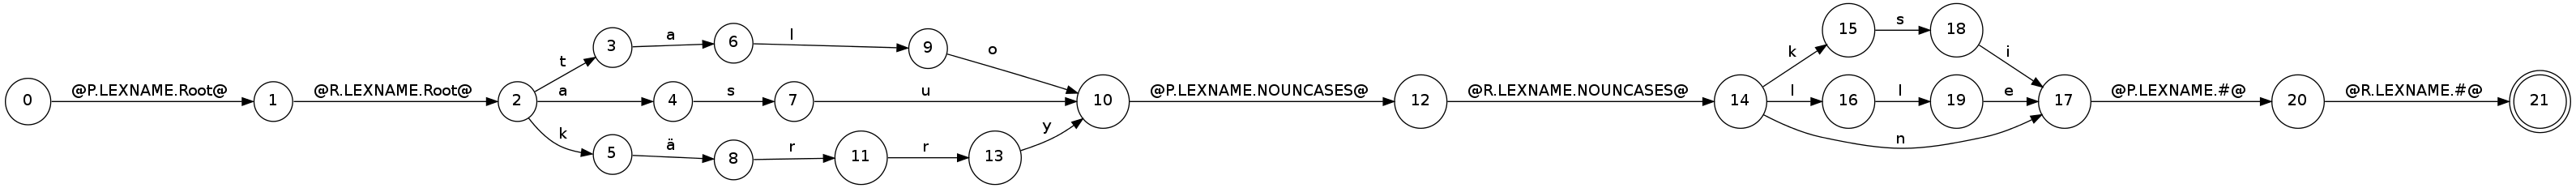
\includegraphics[width=\textwidth]{transducer.png}
     \caption{Simplified part of Finnish lexc grammar description with automatic flags
     \label{fig:lexc-fin-flag}}
\end{figure*}

\begin{figure*}[!htb]
    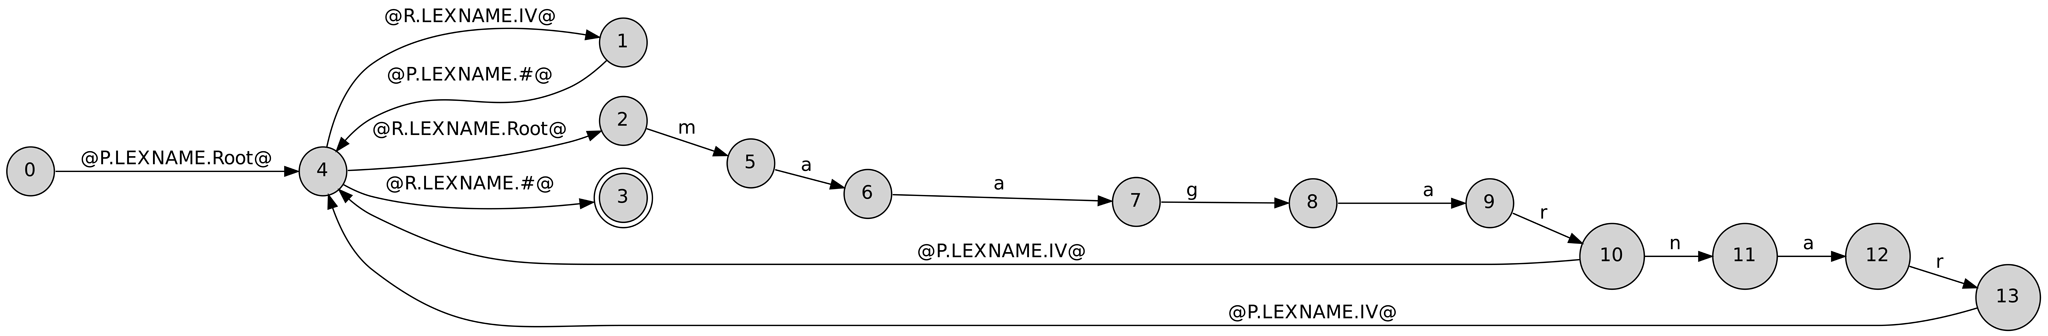
\includegraphics[width=\textwidth]{gr.png}
     \caption{Simplified part of Greenlandic lexc grammar description with automatic flags
     \label{fig:lexc-gr-flag}}
\end{figure*}

\section{Background}
\label{sec:background}

Finite state morphology~\cite{beesley2003finite} is the
state-of-the-art in writing morphological analysers for natural
languages of the whole range of typologically varying morphological
features. The finite-state approach is built around two practical
concepts: constructing lexicographical descriptions of the language
using a syntax called lexc and expressing morphophonological
variations as regular expression rules. In this paper we study lossless
hyper-minimization of finite-state machines derived from lexicographic
descriptions in the lexc formalism \cite{beesley1998constraining}.

Hyper-minimization of minimal deterministic finite-state machines
refers to procedures which produce an even smaller finite-state
machine which preserves some of the qualities of the original
deterministic minimal machine. Hyper-minimization comes in two flavors
lossy and lossless.

Lossy hyper-minimization algorithms~\cite{maletti2011} introduce a
limited amount of changes to the language accepted by the original
machine. This makes the machine susceptible to further size reduction
using conventional minimization algorithms. Lossy hyper-minimization results in a deterministic machine which allows fast lookup.

In contrast to lossy hyper-minimization, the approach presented in
this paper is lossless. We introduce a limited amount of
non-determinism into the finite-state machine using flag
diacritics. Thus we achieve size reduction, while at the same time
preserving the original language accepted by the finite-state
machine. The non-determinism introduced by the algorithm results in
some reduction in run-time during lookup. Nevertheless, our
experiments show that this reduction is not prohibitive in practice
(see Section \ref{results}).

Finding the smallest non-deterministic finite-state machine equivalent
to a given machine is PSPACE complete \cite{jiang1993} for general
finite-state machines and thus intractable. Nevertheless, using a
linguistic description, rather than a compiled finite-state machine,
as starting point it is possible to achieve substantial reduction in
the size of the machine without penalties in compilation time (see
Section \ref{results}).

Our approach is applied to lexicogrphical descriptions in lexc. Lexc
is a simple right-linear phrase structure grammar formalism. In
linguistic terms this means approximately the following: we have
collections of lexicons, which are lists of morphemes. Each morpheme
in a lexicon defines a continuation lexicon, which in turn determines
the set of morphemes that can succeed the original morpheme and their
possible continuations.

Consider for example Finnish morphology. Nominal inflection can be
constructed neatly from left to right. In figure~\ref{fig:lexc-fin},
there is a lexc representation of the Finnish words \emph{talo} `house',
\emph{asu} `clothing' and \emph{kärry} `cart', and nominal suffixes
\emph{n} (singular genitive), \emph{lle} (singular allative) and
\emph{ksi} (singular translative). Derivation of word-forms starts
from the \texttt{Root} lexicon. Each of the nouns in root set of morphemes
continues rightwards to \texttt{NOUNCASES} set of morphemes, and each
case morpheme continues towards the special \texttt{\#} lexicon
signifying the end of a word-form.

\begin{figure}
    \centering
    \begin{verbatim}
    LEXICON Root
    talo NOUNCASES ;
    asu NOUNCASES ;
    kärry NOUNCASES ;

    LEXICON NOUNCASES
    n # ;
    lle # ;
    ksi # ;
    \end{verbatim}
    \caption{Simplified part of Finnish lexc grammar description
    \label{fig:lexc-fin}}
\end{figure}

Finnish was used as an example in Karttunen's paper on flag diacritics
in optimisation~\shortcite{karttunen2006numbers}. In that paper, he
showed that the optimisation quality of wisely selected flag
diacritics can be substantial; from a 20,498 state automaton to an
1,946 state one. The article describes Finnish numerals, which have
the feature of requiring agreeing inflection in free compounding. This
can be achieved by allowing all compounds and restricting the
combinations by flags, instead by lexicon structure. Unfortunately,
the article does not show examples or re-producible description of the
lexicographical data, but to our experience there are no available
morphologies that show similar compression quality, so it can be
considered towards the upper bounds of what such compression can
achieve.

One of the reasons why flag diacritics have been so cumbersome from
the linguists point of view, is their two-fold nature. On one hand,
they are there to optimise the finite-state automaton structure,
e.g. in~\cite{karttunen2006numbers}. On the other hand, they are the
primary method of describing non-contiguous morphological
constraints~\cite{beesley1998constraining}. If they are applied on the
constriction of separated morphotactic dependencies, the effect on
optimisation is at best haphazard, and the resulting description is
neither linguistically motivated nor maintainable from a computational
view-point.

In order to circumvent problems associated with manually applied flag
diacritics, Drobac et al. \shortcite{drobac2014} present an approach
to inducing flag diacritics into lexc lexicons. Our work can be seen
as a refinement of their approach.

We attempt to compare our approach to Drobac et
al. \shortcite{drobac2014}, but direct comparison is difficult for
several reasons. The sizes of the transducer binaries reported by
Drobac et al. \shortcite{drobac2014} are the result of first inducing
flags automatically and then removing some of them in order to reduce
the size of the final machine. We do not remove flags, since it is
time consuming and our approach yields small binaries even without
flag removal. Prior to removing flags, the binary sizes reported by
Drobac et al. \shortcite{drobac2014} are much larger than the sizes we
achieve. We could probably achieve even further size reductions by
removing some of the flags.

The approach taken by Drobac et al. \shortcite{drobac2014} also
requires path filtering if phonological rules are applied to the
lexicon. This is explained in section \ref{methods}. In contrast, our
approach requires no path filtering, which shortens compile time.

\section{Flag diacritics}
\label{sec:flags}

Flag diacritics are special multi-character symbols which are interpreted during runtime. They can be used to optimize large transducers to couple entrance points of the sub-graphs with the correct exit points.

Their special syntax is: \verb+@operator.feature.value@+, where
\texttt{operator} is one of the available operators (P, U, R, D, N, C), \texttt{feature} is the name of a feature set by the user and \texttt{value} can be any value held in a feature, also provisionally defined. For additional information on the semantics of flag diacritic operators, see~\newcite{beesley2003finite}.


In this paper, we will use only two types of flag diacritics: positive
setting (\verb+@P.feature.value@+) and require test
(\verb+@R.feature.value@+). While a positive setting flag only sets the
feature to its value, the require test flag invokes testing whether the
feature is set to the designated value. For example,
\verb+@P.LEXNAME.Root@+ will set feature \texttt{LEXNAME} to value
\texttt{Root}. If later in the path there is an R flag that requires test
\verb+@R.LEXNAME.Root@+, the invoked test will succeed and that path
will be considered valid.


\section{Notation}
\label{sec:notation}
TODO ...


\begin{table}[h]
    \centering
    \begin{tabular}{|c|c|}
        \hline
        \bf Operation & \bf Name \\
        \hline\hline
        \bf a b & concatenation  \\
        \bf a | b & disjunction  \\
        \bf a : b & cross product  \\
        \bf a .o. b & composition  \\
        \bf * & Kleene star  \\
        

        \hline
    \end{tabular}
    \caption{List of operators
    \label{table:operators}}
\end{table}




\section{Methods}
\label{sec:methods}


\begin{figure}[htbp]
    \centering

\begin{subfigure}[t]{0.3\textwidth}
\begin{verbatim}
LEXICON Root
A ;
B ;
C ;

LEXICON A
aaa A ;
# ;

LEXICON B
aaaa B ;
# ;

LEXICON C
aaaaa C;
#;
\end{verbatim}
\caption{Lexc grammar description
\label{fig:lexc-a2}}
\end{subfigure}
 ~ %add desired spacing between images, e. g. ~, \quad, \qquad etc.
\begin{subfigure}[t]{0.3\textwidth}
\begin{verbatim}
ORIGINAL:
no. of states: 60
no. of arcs: 60
no. of final states: 36
\end{verbatim}
\caption{Summary of the transducer without flag diacritics
\label{fig:sizes-orig}}
\end{subfigure}%
 ~ %add desired spacing between images, e. g. ~, \quad, \qquad etc.
\begin{subfigure}[t]{0.3\textwidth}
\begin{verbatim}
HYPER-MINIMAL:
no. of states: 23
no. of arcs: 27
no. of final states: 1
\end{verbatim}
\caption{Summary of the hyper-minimal transducer
\label{fig:sizes-flags}}
 \end{subfigure}

 \caption{Simple example lexicon with transducer sizes}
 \label{fig:simple-ex}
\end{figure}


This algorithm is an improvement of the hyper-minimization algorithm introduced in~\newcite{drobac2014}. The main idea of the algorithm is to 
replicate the structure of a morphological lexicon into a finite state transducer with the use of flag diacritics. Every sub-lexicon should start 
with a require flag \verb+R.LEXNAME.sub-lex+, where \verb+LEXNAME+ is the feature name that we use for this special purpose
and \verb+sub-lex+ is the name of the current sub-lexicon. Accordingly, every continuation should be expressed with positive setting flag 
\verb+P.LEXNAME.sub-lex+, which sets feature \verb+LEXNAME+ to a \verb+sub-lex+ value, which corresponds to the continuation lexicon.
TODO - example?

\begin{figure}
\centering
\begin{subfigure}[b]{0.4\textwidth}
        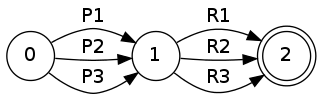
\includegraphics[width=\textwidth]{hub.png}
        \caption{A hub state}
        \label{fig:hub}
\end{subfigure}%
\quad %add desired spacing between images, e. g. ~, \quad, \qquad etc.
  %(or a blank line to force the subfigure onto a new line)
\begin{subfigure}[b]{0.4\textwidth}
        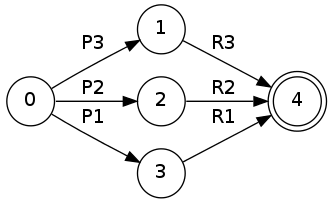
\includegraphics[width=\textwidth]{distr.png}
        \caption{Distributed hub}
        \label{fig:distr}
\end{subfigure}
\caption{Hub state before and after distribution}
\label{fig:hub_distr}
\end{figure}


While in the previous version flags were concentrated in flag diacritic hubs, single states in which all continuation lexicons end with positive settings and from which they continue with a require test, in the new method, flag diacritic states are distributed. For example, if one hub state would have incoming transitions 
$P_1$, $P_2$, $P_3$ and outgoing transitions $R_1$, $R_2$, $R_3$, the distributed version would be divided into three states, each with one 
$P_i$ $R_i$ pair, as shown in 
Figure~\ref{fig:hub_distr}. Therefore, we can say:

\begin{equation}\label{hub_replacement}
[P_1 | P_2 | P_3] [R_1 | R_2 | R_3] \rightarrow [P_1 R_1] | [P_2 R_2] | [P_3 R_3]
\end{equation}



This distributiveness is necessary because it allows 
composition of lexicon with grammar rules without creating extra invalid flag diacritic paths, which means that, 
unlike in the previous version, there is no need for pruning paths with invalid flag combinations after the composition.


One of the examples why preserving the lexical structure with flag diacritics is useful is explained on a small-scale artificial example shown in 
Figure~\ref{fig:simple-ex}.
 
The Figure~\ref{fig:lexc-a2} shows the language description of the following language: $(aaa)^*|(aaaa)^*|(aaaaa)^*$, written in 
the \texttt{lexc} format. In case this language is compiled into a normal, minimal transducer, it will consist of 60 states and 60 arcs, 
but with the hyper-minimal method, the transducer size will be less then half of it: 23 states and 27 arcs, as shown in 
Figure~\ref{fig:sizes-orig} and Figure~\ref{fig:sizes-flags} respectively.

This happens because the non-flagged transducer will try to combine and keep all possible options of strings in the same path, until it gets 
the least common multiple of strings $aaa$, $aaaa$ and $aaaaa$. On the other hand, the flagged version will be able to distribute those three 
strings into different paths, avoiding duplication as much as possible.

If we define transducer depth as the length of the longest path from any state to another state that does not go through the same state twice, 
the non-flagged version has a maximal depth of 59 after which it returns to the starting state to complete the cycle, while the hyper-minimal 
one has the maximal depth of 9. Keeping the transducer shallow will reduce the necessary number of states and paths, which results in a smaller final size.

Similar combinatorial phenomena occur in large lexicons, like in Greenlandic, but it is difficult to find illuminating and small real 
world examples that can be presented in a paper.


\begin{figure*}
    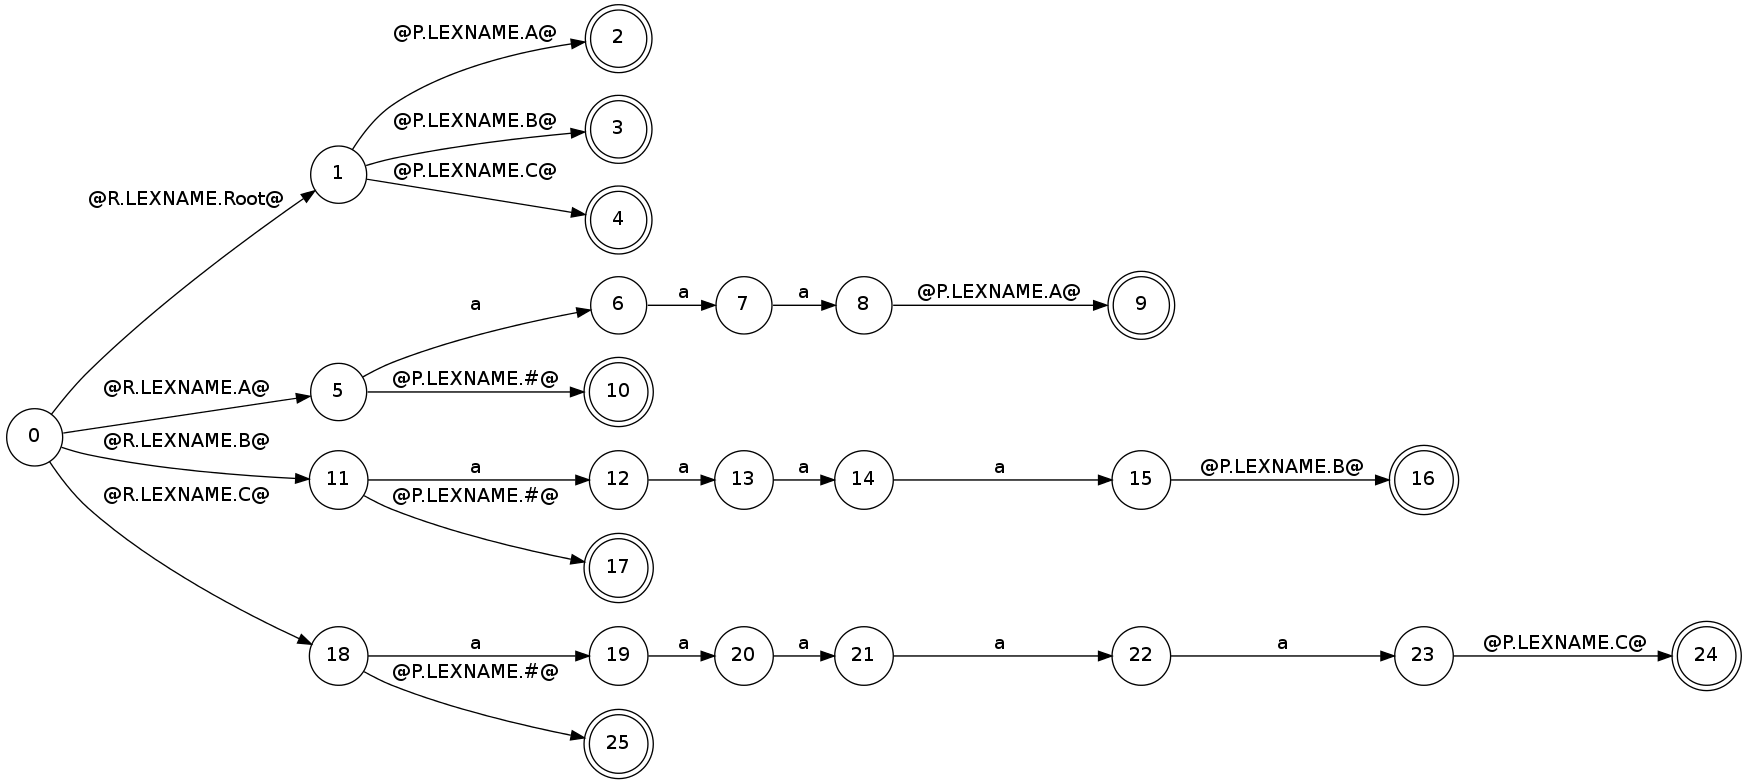
\includegraphics[width=\textwidth]{trie.png}
     \caption{First step is to build a lexical trie
     \label{fig:trie}}
\end{figure*}


\begin{figure*}
    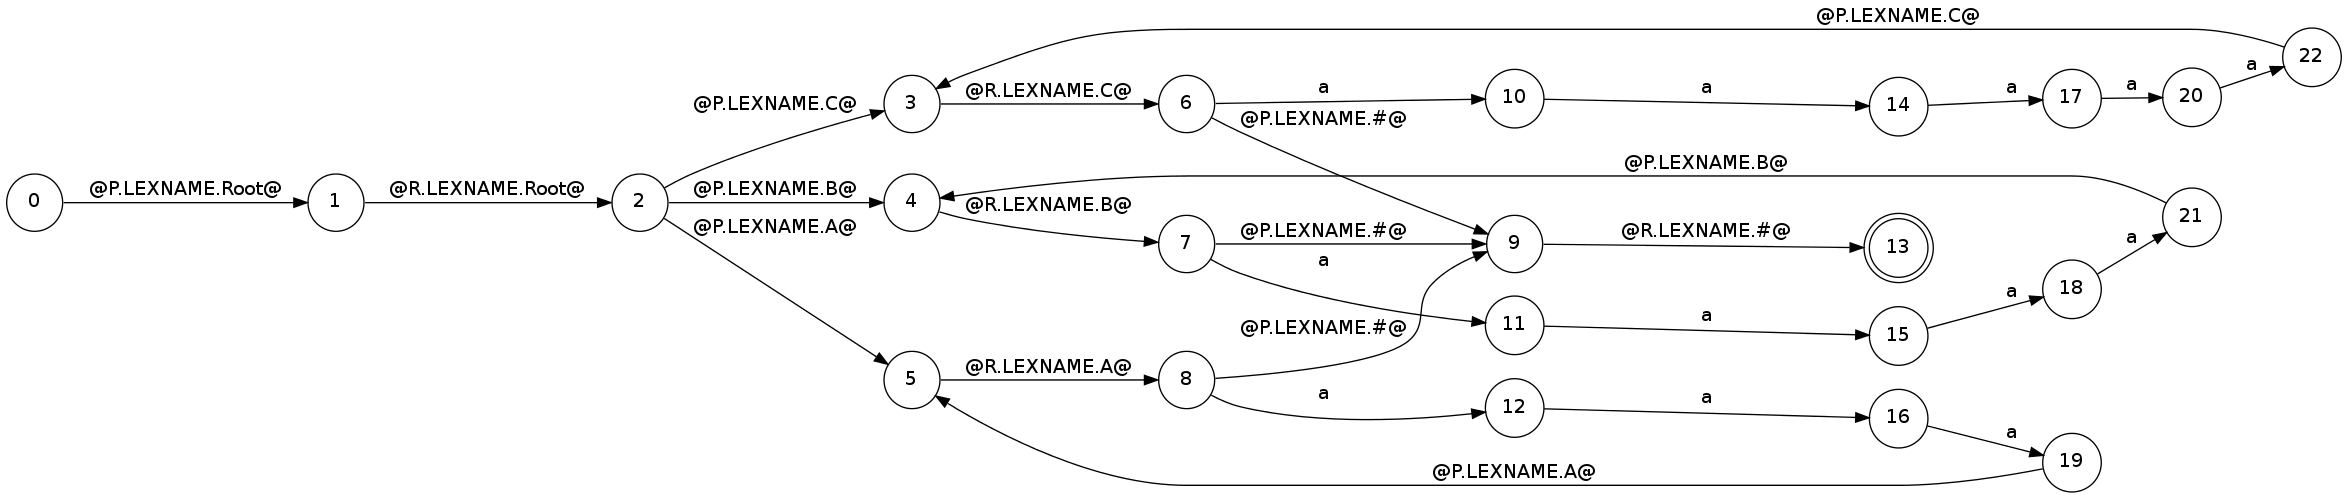
\includegraphics[width=\textwidth]{after_comp.png}
     \caption{Transducer after composition with filter
     \label{fig:after}}
\end{figure*}



\subsection{Lexical compilation}

Previous version of \texttt{lexc} took too long to compile because each sub-lexicon was built separately and then disjuncted with others. The compilation time of large morphologies would take up to several hours. In order to improve compilation speed and incorporate hyper-minimization, we needed to change the \texttt{lexc} algorithm.

First, from a lexical description, we build a transducer trie, an ordered, acyclic finite-state transducer. In the trie, every sub-lexicon 
starts from the same start state with a require flag with a sub-lexicon name as a value. After the require flag, the morph continues, followed 
by a positive setting flag with a continuation value. In the case where the morph is a pair of two strings, epsilon padding is added to the end of 
the shorter string.

\texttt{Lexc} can also contain regular expressions. In that case, the regular expression is parsed and processed into a transducer which is saved into 
a map of regular expression keys and matching transducers. The key is added to the trie in the same way as the strings are, i.e. the trie entry will start with 
the encoded sub-lexicon name, followed by the regular expression key and finish with the continuation. Later in the process, the regular expression 
keys are substituted with matching transducers from the map. 
Example of a trie built from the lexical description in Figure~\ref{fig:lexc-a2} is shown in Figure~\ref{fig:trie}.

When the entire lexical file is read into a trie, the trie is transformed into a transducer and over-generated with Kleene star:
\begin{equation}\label{eq:trie_star}
tr = \left[f(trie)\right]^* 
\end{equation}
Transformation of the trie to a transducer is a fast operation, even for large data structures, which also gives us a fast and efficient version of \texttt{lexc}.

The next step is concatenation of start and end encoded joiners with the beginning and the end of the transducer. 
%(In case of non-flagged version, the starting joiner is initial lexicon name, usually \texttt{Root} and ending joiner is encoded final lexicon, \texttt{\#}.)
For the hyper-minimized transducer, the starting joiner is the \verb+P+ flag of the initial sub-lexicon, usually \texttt{P.LEXNAME.Root} and the ending joiner is the \verb+R+ flag of the final lexicon, \texttt{R.LEXNAME.\#}.

\begin{equation}\label{eq:joiners}
tr' = \verb+P.LEXNAME.Root + tr \verb+ R.LEXNAME.#+
\end{equation}
This ensures that the transducer always starts and ends with the same flag pair.

To filter out invalid flag diacritic paths, caused by trie over-generation from equation~\ref{eq:trie_star}, the transducer is composed with a filter:
\begin{equation}\label{eq:composition}
tr'' = tr' .o. filter
\end{equation}
where the filter is:
\begin{equation}\label{eq:filter}
filter = \left[ \left(\bigcup_{i} \verb+P.LEXNAME+_i \verb+ R.LEXNAME+_i \right) \cup (\Sigma \setminus F) ^*\right]^* 
\end{equation}

and $(\Sigma \setminus F)^*$ denotes universal language without the hyper-minimization \verb+P+ and \verb+R+ flags.


In case the user wishes to remove some flag pairs from the transducer, they can be replaced with epsilon at this point.


The final step when constructing the lexc transducer is to replace regular expression keys with actual regular expression transducers
\begin{equation}\label{eq:regex}
regular\_expession\_key \rightarrow regular\_expression\_transducer
\end{equation}

In Figure~\ref{fig:after}, we show the final hyper-minimal transducer built from the lexical description in Figure~\ref{fig:lexc-a2}. 



\section{Data}
\label{sec:data}

We measure the success of our algorithm using real-world, large-scale
language descriptions. For this purpose we have acquired freely
available, open source language descriptions from the language repository of the University of 
Tromssa~\cite{moshagen2013building}.\footnote{https://victorio.uit.no/langtech, revision 90691} The
languages selected are Greenlandic (kal), North Saami (sme), Erzya
(myv), Finnish (fin) and Lule Sami (smj).

All operations with transducers were performed using Helsinki Finite
State Technology tools~\cite{linden2011}.\footnote{svn.code.sf.net/p/hfst/code, revision 3813}



\section{Results}
In Table~\ref{table:sizes}, we show the sizes of the morphological analyzers built with different approaches. The first column shows analyzer 
size without any flag diacritics, it is followed by the sizes achieved with the previous method and finally there are sizes when 
compiled with the method proposed in this paper.
\begin{table}
    \centering
    \begin{tabular}{|l|r|r|r|r|r|}
        \hline
        \bf Language & \bf Original & \bf Old flags  & \bf \% & \bf New flags  & \bf \% \\
        \hline\hline
        \bf Greenlandic &   168 M  & 17 M & 10,1\% &  14 M & 8,3\% \\
        \bf North Saami &   12 M    & 5,7 M & 47,5\% & 10 M & 83,3\% \\
        \bf Finnish &   17 M    & 16 M & 94,1\% & 16 M & 94,1\% \\
        \bf Lule Saami  &   5 M    & 3 M & 60,0\% & 5 M & 100\% \\
        \bf Erzya       &   3,7 M    & 5,3 M & 143,2\% &  5 M & 135,13\% \\
        \hline
    \end{tabular}
    \caption{Analyzer size - Sizes of transducers without and with automatic flags (in megabytes); Percentage shows size of the flagged transducer in comparison with the original
    \label{table:sizes}}
\end{table}

In Table~\ref{table:lookup} we show lookup speed of the morphological analysers expressed in words per second...

\begin{table}[h]
 \centering
    \begin{tabular}{|l|r|r|r|r|r|}
        \hline
        \bf Language & \bf Original & \bf Old version & \bf \% & \bf New version & \bf \% \\
        \hline\hline
        \bf Greenlandic & 2 770 w/s & 2 507 w/s & 90,5\% & 2072 w/s & 74,8\%  \\
        \bf North Saami & 30 714 w/s & 8 775 w/s & 28,6\% & 11 168 w/s & 36,4\%  \\
        \bf Finnish  & 84 415 w/s & 27 420 w/s & 32,5\%  & 28 615 w/s & 33,9\%  \\
        \hline
    \end{tabular}
    \caption{Look-up speed of transducers without and with automatic flags; Percentage shows speed of the flagged transducer in comparison with the original
    \label{table:lookup}}
\end{table}


% Find out and discuss why tr with lots of flags get big after applying rules



\section{Discussion}
\label{sec:discussion}



%\subsection{Future Directions}
%\label{subsec:future-directions}

%This is an optimistic thing so we thought that automatic induction of flags
%shoulda work nicely for other neat things too. Hyper-minimization based on
%morphophonology would be cool. Also, graph-structure. And other things.

\section{Conclusion}
\label{sec:conclusion}



\iffalse
\section*{Acknowledgements}
The research leading to these results has received funding from FIN-CLARIN, Langnet and the
European Commission's 7th Framework Program under grant agreement n° 238405 (CLARA).
\fi

\bibliographystyle{acl}
\bibliography{hyperminimization-with-lexc2.bib}




\end{document}


